\documentclass[a4paper,12pt]{article}
\usepackage[a4paper]{geometry}
\usepackage{polski}
\usepackage[polish]{babel}
\usepackage[utf8]{inputenc}
\usepackage{indentfirst}
\usepackage{graphicx}
\usepackage{lastpage}
\usepackage{fancyhdr}
\usepackage{hyperref}
\usepackage{float}
%head & foot
\pagestyle{fancy}
\title{Specyfikacja implementacyjna projektu \textit{Gra w Życie} w~języku C}
\author{Chabik Jan (291060), Łuczak Mateusz (291088)}
\date{15 marca 2018}
\setlength\parindent{24pt}
\setlength{\headheight}{16pt}
\lhead{}
\rhead{Specyfikacja implementacyjna projektu \textit{Gra w Życie} w języku C}
\rfoot{str. \thepage/\pageref{LastPage}}
\cfoot{}

\begin{document}
\maketitle
\thispagestyle{empty}
\begin{center}
	
\includegraphics[scale=0.1]{logo_ee_big.png}
\end{center}
\newpage

\tableofcontents
\pagenumbering{arabic}
\newpage

\section{Diagram modułów}
\subsection{Diagram}
\begin{center}
	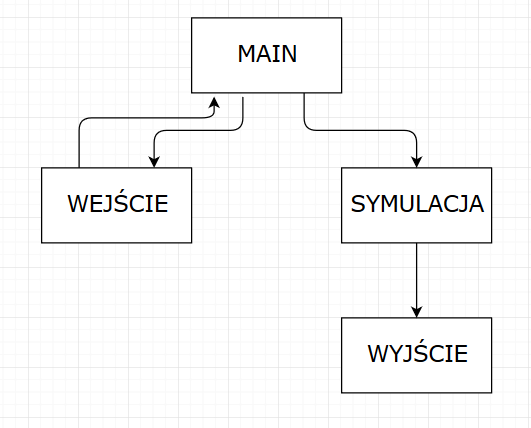
\includegraphics[scale=1]{diagram.png}
\end{center}
\subsection{Opis diagramu}
\begin{itemize}
\item \texttt{MAIN} - Główna funkcja programu. Przekazuje dane do funkcji sprawdzającej wejście, tworzy macierze dla mapy automatu komórkowego i wysyła parametry wejścia do modułu \texttt{SYMULACJA};
\item \texttt{WEJŚCIE} - Funkcja sprawdzająca parametry wejścia, wyświetla odpowiednie komunikaty o błędach i wysyła informacje do funkcji głównej;
\item \texttt{SYMULACJA} - Funkcja odpowiadająca za generowanie nowych map automatu komórkowego na podstawie poprzedników i reguł sąsiedztwa. Odpowiednie dane (mapa, numer generacji, katalog wyjściowy) są wysyłane do modułu \texttt{WYJŚCIE};
\item \texttt{WYJŚCIE} - Funkcja odpowiadająca za wypisanie danych wynikowych w formatach \texttt{.txt} i \texttt{.png} do przygotowanego katalogu. Na życzenie użytkownika, wypisuje również informacje do terminala.
\end{itemize}
\section{Funkcje}
\subsection{Funkcje modułu głównego}
\begin{itemize}
\item \texttt{INIT\_MATRIX} - funkcja tworząca macierze, które będą przechowywać dane dotyczące mapy automatu komórkowego. Zostaną one utworzone natychmiastowo po sprawdzeniu danych wejściowych i wczytaniu wymiarów mapy automatu.
\end{itemize}
\subsection{Funkcje modułu wejścia}
\begin{itemize}
\item \texttt{CHECK} - funkcja interpretująca informacje dotyczące danych wejściowych:
	\begin{itemize}
	\item \texttt{CHECK\_INPUT\_FILE} - funkcja sprawdzająca plik wejściowy \texttt{.txt} pod względem błędów odczytu lub błędów pliku;
	\item \texttt{CHECK\_OUTPUT\_CATALOG} - funkcja sprawdzająca katalog wyjściowy pod względem błędów zapisu (ewentualny brak dostępu do katalogu);
	\item \texttt{CHECK\_ARGS} - funkcja sprawdzająca argumenty podane przez użytkownika podczas uruchamiania programu.
	\end{itemize}
\end{itemize}
\subsection{Funkcje modułu symulacji}
\begin{itemize}
\item \texttt{MAINF} - Funkcja wywołująca wybraną ścieżkę na podstawie wybranego sąsiedztwa i opcji dialogowej. Po zakończeniu generowania nowej mapy, jest ona kopiowana w miejsce jej poprzednika (do pierwszej macierzy);
\item \texttt{SASIEDZTWOM} - Funkcja obsługująca sąsiedztwo Moore'a;
\item \texttt{SASIEDZTWON} - Funkcja obsługująca sąsiedztwo von Neumanna.
\end{itemize}
\subsection{Funkcje modułu wyjścia}
\begin{itemize}
\item \texttt{OUTPUT\_TO\_TERM} - Funkcja, która wypisuje dane do terminala i obsługuje dialog z użytkownikiem, który ma wybór pomiędzy zapisem aktualnej generacji do pliku \texttt{.png}, lub jego pominięciem. Zapis do pliku \texttt{.txt} jest automatyczny i użytkownik nie może wybrać, czy generacja ma zostać pominięta. Dzięki temu, zapisane zostają wszystkie generacje i użytkownik może wywołać program dla wybranego pliku \texttt{.txt}. W innym wypadku, istniałoby ryzyko, gdzie nie zostałyby zapisane żadne pliki w formacie tekstowym oraz niemożliwe byłoby przywrócenie wybranej generacji bez tworzenia ich raz jeszcze;
\item \texttt{MAIN\_OUTPUT} - Funkcja zapisująca dane do pliku \texttt{.txt} oraz \texttt{.png}.
\end{itemize}
\section{Metodyka wersjonowania}
\begin{itemize}
\item Wersjonowanie oprogramowania następuje na systemie kontroli wersji Git;
\item Każda z części kodu jest udostępniana na nowych gałęziach (\textit{branch});
\item Wersje dokumentów obarczone będą nazwą z dopiskiem \texttt{beta} lub \texttt{FINAL}, oraz numerem wersji:
	\begin{itemize}
	\item \texttt{beta} - robocza wersja dokumentu;
	\item \texttt{FINAL} - ostateczna wersja dokumentu;
	\item numer wersji - numer oznaczający aktualną kompilację. Określony zostaje w formacie X.Y, gdzie X to numer kompilacji, a Y numer poprawki. Y jest opcjonalne i występuje tylko przy małych zmianach w dokumencie (takich jak przykładowo poprawa literówki).
	\end{itemize}
\item Wersje dokumentów obarczone będą nazwą z dopiskiem \texttt{beta} z numerem kompilacji w razie wysłania do repozytorium wersji roboczej,  \texttt{FINAL} w przypadku wersji ostatecznej. W przypadku dodatkowych poprawek, będzie posiadać numer kompilacji.
\end{itemize}

\section{Kompilator i wersja języka}
\subsection{Kompilator}
Używanym kompilatorem będzie \texttt{gcc}. Dzięki niemu możliwe jest dobranie wersji języka C. Jest to również kompilator ogólnodostępny i darmowy.
\subsection{Wersja języka}
Wybraną wersją języka C jest \texttt{C99} ze względu na dodatkowe udogodnienia przy pisaniu kodu. Jednym z przykładów może być możliwość deklarowania zmiennej podczas tworzenia pętli \texttt{for}.

\noindent
Przykład:
\begin{center} 
\texttt{for(int i=0;i<10;i++) /* kod */}
\end{center}

Do kompilacji kodu w tym standardzie konieczne jest użycie flagi \texttt{-std=c99}.

\noindent
Przykład:
\begin{center}
\texttt{gcc -std=c99 foo.c}
\end{center}

\section{Użyte biblioteki}
\begin{itemize}
\item \texttt{png.h} - obsługa obrazów w formacie \texttt{.png}. Do użycia konieczne jest doinstalowanie biblioteki \texttt{libpng}, która jest dostępna do pobrania pod adresem: \url{https://libpng.sourceforge.io/index.html}
\end{itemize}

\section{Testowanie i konwencja}
\subsection{Testowanie}
Testy zostaną wykonane przez nas ręcznie. Testować będziemy każdą funkcję z osobna, a potem każdy moduł. 

\subsection{Konwencja}
Będziemy testować program przez napisanie funkcji przypisanych do poszczególnych funkcjonalności. Zamiast jednej funkcji sprawdzającej działanie modułu wejścia, napiszemy takich funkcji wiele i każda z nich będzie testować jedną, unikatową funkcjonalność (np. poprawny komunikat przy problemie z plikiem wejścia, funkcja będzie się nazywać \texttt{shouldShowInputFileError()} ). Robimy tak, by jak najszybciej identyfikować błędy w naszym kodzie.

\subsection{Kontrola wycieków pamięci}
Do kontroli wycieków pamięci będziemy używać programu \texttt{Valgrind}. Jest to program łatwy w obsłudze, skuteczny i darmowy. Pozwala sprawdzić, w którym miejscu następuje wyciek, oraz ile danych zostaje utraconych.
\end{document}
